\documentclass{article}
\usepackage{tikz}
\usetikzlibrary{automata, positioning, arrows}
\begin{document}
\pagestyle{empty}
\begin{figure}[ht]
\centering

  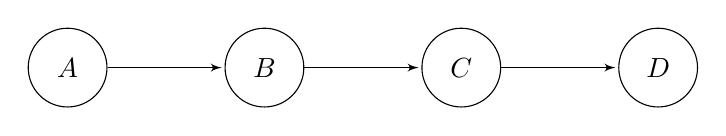
\begin{tikzpicture}[>=latex', shorten >=1pt, auto,
    node distance=2.5cm, scale=1,
      transform shape, align=center]

    \tikzset{
      vertex/.style = {shape=circle,draw,minimum size=1cm},
    }

    \node[vertex            ] (A) {$A$};
    \node[vertex, right of=A] (B) {$B$};
    \node[vertex, right of=B] (C) {$C$};
    \node[vertex, right of=C] (D) {$D$};

    \path[->]
    % die wirklich essentiellen
      (A) edge[] (B)
      (B) edge[] (C)
      (C) edge[] (D);

  \end{tikzpicture}

\end{figure}
\end{document}
